\begin{graphicspathcontext}{{./chapters/mas/examples/imgs/auto/},\old}

\sidenote{\cite{Russell.20}, Image Clause Sonet 4.6}
\begin{frame}{Definition of the Vacuum World}
	\begin{columns}
		\begin{column}[t]{.5\linewidth}
			\begin{block}{Environment}
				\begin{itemize}
				\item A grid of \emph{rooms}, each of which is either \emph{Clean} or \emph{Dirty}
				\item One (or more) \emph{vacuum robot(s)} occupying a room at a time
				\end{itemize}
			\end{block}
			\begin{block}{Agent}
				\begin{description}
				\item[Perceives] \texttt{Dirty}, \texttt{Clean}, \texttt{CanGoLeft}, \texttt{CanGoRight}, \texttt{CanGoUp}, \texttt{CanGoDown}
				\item[Acts] \texttt{Suck}, \texttt{MoveLeft}, \texttt{MoveRight}, \texttt{MoveUp}, \texttt{MoveDown}
				\end{description}
			\end{block}
		\end{column}
		\begin{column}[t]{.5\linewidth}
			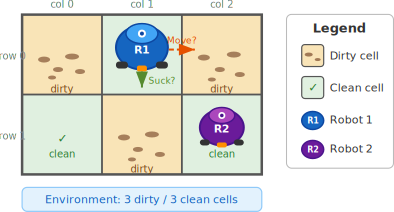
\includegraphics{vacuum_world} \\[.5cm]
			\begin{block}{Possible Performance Measure}
			Maximise the \emph{number of clean cells} over time, minimising energy consumption
			\end{block}
		\end{column}
	\end{columns}
\end{frame}

\begin{frame}[fragile]{Vacuum Agent Loop}
	\begin{columns}
		\begin{column}{.5\linewidth}
				\begin{sarllisting}
def run() {
	var done = false
	while (!done) {
	  var p = get_percept()
	  var a = choose_action(p)
	  do_action(a)
	  done = check_if_done()
	}
	die()
}\end{sarllisting}
		\end{column}
		\begin{column}{.5\linewidth}
			\begin{block}{\texttt{get\_percept()}}
				Convert sensor data to the logical facts for perceptions
			\end{block}
			\begin{block}{Reactive behavior: \texttt{choose\_action()}}
				If the current cell is dirty, suck \\
				Otherwise, move \\[1ex]
				\centering
				\begin{tabular}{|c|c|}
				\hline
				\textbf{Perception \texttt{p}} & \textbf{Action \texttt{a}} \\
				\hline
				\texttt{[Dirty]} & \texttt{Suck} \\
				\hline
				\texttt{[Clean, CanGoLeft]} & \texttt{MoveLeft} \\
				\hline
				\texttt{[Clean, CanGoRight]} & \texttt{MoveRight} \\
				\hline
				\texttt{[Clean, CanGoUp]} & \texttt{MoveUp} \\
				\hline
				\texttt{[Clean, CanGoDown]} & \texttt{MoveDown} \\
				\hline
				\end{tabular}
			\end{block}
		\end{column}
	\end{columns}
\end{frame}

\begin{frame}[fragile]{Vacuum Agent Loop \insertcontinuationtext}
	\begin{columns}
		\begin{column}{.5\linewidth}
				\begin{sarllisting}
def run() {
	var done = false
	while (!done) {
	  var p = get_percept()
	  var a = choose_action(p)
	  do_action(a)
	  done = check_if_done()
	}
	die()
}\end{sarllisting}
		\end{column}
		\begin{column}{.5\linewidth}
			\begin{block}{\texttt{do\_action()}}
				Convert selected action fact to a concrete effect with the robot effectors
			\end{block}
			\begin{block}{\texttt{check\_if\_done()}}
				Determine if the robot has to stop its running
			\end{block}
			\begin{block}{Does this agent perform well?}
				\smaller Need a performance measure:
				\begin{compactitemize}
				\item Maximize amount of dirt picked up?
				\item Maximize ratio of dirt to energy expended?
				\item Maximize ratio of dirt to combination of energy and time?
				\end{compactitemize}
				Selecting a performance measure is not always easy
			\end{block}
		\end{column}
	\end{columns}
\end{frame}

\end{graphicspathcontext}

\endinput

